\documentclass[a4paper,10pt]{article}
\usepackage[utf8]{inputenc}
\usepackage[T1]{fontenc}
\usepackage[francais]{babel}
\usepackage[a4paper,top=2.5cm, bottom=2.5cm, left=2.5cm, right=2.5cm]{geometry}
\usepackage{longtable}
\usepackage[final]{pdfpages} 


%opening
\title{INFO-F-403 : Language theory and compiling \\ Rapport projet partie 3 - Génération de code}
\author{Simon Picard \\ Arnaud Rosette}

\begin{document}

\maketitle
\clearpage
\tableofcontents
\clearpage

\section{Introduction}
Dans cette partie du projet, il nous est demandé de modifier la grammaire donnée dans l'énoncé afin de rendre celle-ci LL(1). Il faut donc appliquer toute une série de règles et d'algorithmes pour rendre cette grammaire moins ambigüe et LL(1), dans le but de construire ``l'action table'' à partir des ensembles first et follow. L'inclusion des fonctions dans la grammaire fait partie d'un bonus que nous avons décidé de réaliser.

\section{Transformation de la grammaire donnée}
\subsection{Opérateurs binaires et unaires}
La première étape pour rendre la grammaire LL(1) fut la distinction des deux types d'opérateurs : les opérateurs binaires qui agissent sur deux expressions l'une située à gauche et l'autre à droite de ces opérateurs et les opérateurs unaires qui agissent sur une seule expression située à droite de ces opérateurs. Il faut différencier les deux types d'opérateurs afin de ne pas avoir des expressions du style : >>4, *2, 6|,... .Les opérateurs unaires sont au nombre de quatre : ! (negation), $\sim$ (not bit à bit), + et -. Les opérateurs + et - sont également des opérateurs binaires. 
\subsection{Priorité et associativité des opérateurs}
Lors de cette étape, nous avons modifié la grammaire afin de fixer la priorité et l'associativité des différents opérateurs, ceci afin de rendre la grammaire moins ambigüe. Nous avons remarqué que les opérateurs unaires étaient plus prioritaires que les opérateurs binaires et que les opérateurs unaires étaient tous associatifs à droite, tandis que les opérateurs binaires l'étaient tous à gauche. Pour fixer la priorité, nous avons mis les opérateurs les moins prioritaires le plus ``haut'' possible dans la grammaire et les plus prioritaires le plus ``bas'' possible. 
Dans la grammaire ci-dessous où le ``start symbol'' est E, l'opérateur ``+'' est considéré comme plus ``haut'' que l'opérateur ``*'' dans la grammaire car il est possible d'obtenir l'opérateur ``+'' en utilisant moins de règles de production à partir du ``start symbol'' que pour obtenir l'opérateur ``*''.
\begin{verbatim}
E->E + T
 ->T
T->T * F
 ->F
F->ID
 ->( E )
\end{verbatim}

\subsection{Suppression des récursions à gauche}
L'étape suivante fut l'étape de suppression des récursions à gauche qui sont incompatibles avec les ``top-down parser'' car cela fait entrer ce genre de parser dans une boucle ou récursion infinie. Cette étape rend tout opérateur associatif à droite si l'on ne fait rien pour résoudre ce problème lors de l'analyse sémantique.
\subsection{Left factoring}
Cette étape rassemble les règles de production d'une variable qui ont un préfixe commun en une seule règle de production qui contient ce préfixe commun et une nouvelle variable. Cette nouvelle variable possède des règles de production vers les différents suffixes qui étaient présents à l'origine dans les différentes règles de production qui ont été mises en commun. Ceci est nécessaire car le parser qu'on va créer est LL(1), il faut donc qu'il puisse choisir la bonne règle de production en regardant seulement le prochain token qui est en entrée.
\subsection{Les variables <Instruction> et <InstructionList>}
Dans la grammaire donnée, à chaque fois que la variable <Instruction> se trouvait dans la partie droite d'une règle de production excepté lorsque la partie gauche de la règle était <InstructionList>, il y avait une autre règle de production pour cette même partie gauche où <Instruction> était remplacé par <InstructionList>. Par exemple, <If>$\rightarrow$<Expression> <Empty> <InstructionList> <IfEnd> et <If>$\rightarrow$<Expression> <Empty> <Instruction> <IfEnd>. Ceci permettant de ne pas mettre de END\_OF\_INSTRUCTION à la fin d'une <Instruction> lorsque le corps d'un block (ici, le corps du ``if'') ne contenait qu'une seule <Instruction>. 
Le problème posé par le doublement systématique des règles de production contenant des instructions (une règle pour <Instruction> et une autre pour <InstructionList>) est que ce n'est pas factorisé à gauche et que le first de <InstructionList> peut être <Instruction>. 
Afin de résoudre ce problème, nous avons décidé de ne plus utilisé que la variable <InstructionList> dans les autres règles de production. Ainsi, on évite le doublement des règles de production.
Une <InstructionList> est une liste d'<Instruction> séparées par des END\_OF\_INSTRUCTION, avec la dernière <Instruction> qui n'est pas nécessairement suivie d'un END\_OF\_INSTRUCTION. Ceci permet d'avoir un programme du style : if(a>b);a=10 end;
Donc seule une <InstructionList> permet de produire des <Instruction>.
De plus, vu qu'une <InstructionList> peut contenir des instructions vide (une instruction contenant seulement END\_OF\_INSTRUCTION) la variable <Empty> n'est plus nécessaire car celle-ci servait uniquement à indiquer qu'il fallait au moins un terminal END\_OF\_INSTRUCTION.
\subsection{Fonctions}
Les fonctions amènent deux types d'instructions en plus : les définitions de fonction et les appels de fonction. Les appels sont considérés comme des expressions atomiques afin de pourvoir mettre des appels de fonction au sein d'une expression. Par exemple, a=foo()+5;
De plus, il faut qu'une fonction puisse être appelée sans avoir besoin de faire une assignation ou un autre type d'instruction car une fonction peut ne rien retourner et simplement avoir un effet de bord. Par exemple, la fonction println est une fonction qui ne retourne rien mais produit un effet de bord qui est l'affichage dans le terminal. Il faut donc pouvoir faire, par exemple, println(a). C'est pour cela qu'il faut qu'un appel de fonction soit une instruction à part entière.
\subsection{Instructions commencant par un identifier}
Plusieurs instructions commencent par un identifier. Il s'agit des assignations, des déclarations de variables et des appels de fonctions. Afin que la grammaire soit LL(1) il faut factoriser ces instructions. C'est pour cela que la variable <IdentifierInstruction> a été créée. Celle-ci représente une instruction qui commence par un identifier. La variable <IdentifierInstructionTail> a été également créée afin de distinguer les différents types d'instructions qui commencent par un identifier. La distinction est après aisément faite car lorsque le symbole suivant l'identifier est ``='', on sait que c'est une assignation, lorsque ce symbole est ``::'', on sait que c'est une déclaration de variable et lorsque que ce symbole est ``('', on sait que c'est un appel de fonction.
\subsection{Automatisation}
Nous avons développé une série d'algorithm qui permettent de supprimer la reccurssion à gauche, de factoriser à gauche, de supprimer les symboles inutiles et de générer une table d'action ce qui nous permet de vérifier si une grammaire est bien LL(1) via l'action table ou de nous aider à la transformer en grammaire LL(1) grçace aux autres algorithmes.


\section{Grammaire}

Voici la grammaire donnée dans l'énoncé et transformée en grammaire LL(1). A chaque règle de production correspond un numéro qui identifie cette règle.

\begin{longtable}{llll}
$[1]$&<Program>&$\rightarrow$&\begin{tabular}[t]{@{}l@{}}<InstructionList> \end{tabular}\\
$[2]$&<Instruction>&$\rightarrow$&\begin{tabular}[t]{@{}l@{}}<IdentifierInstruction> \end{tabular}\\
$[3]$&&$\rightarrow$&\begin{tabular}[t]{@{}l@{}}<ConstDefinition> \end{tabular}\\
$[4]$&&$\rightarrow$&\begin{tabular}[t]{@{}l@{}}<Block> \end{tabular}\\
$[5]$&&$\rightarrow$&\begin{tabular}[t]{@{}l@{}}<Loop> \end{tabular}\\
$[6]$&&$\rightarrow$&\begin{tabular}[t]{@{}l@{}}<BuiltInFunctionCall> \end{tabular}\\
$[7]$&&$\rightarrow$&\begin{tabular}[t]{@{}l@{}}<FunctionDefinition> \end{tabular}\\
$[8]$&<InstructionList>&$\rightarrow$&\begin{tabular}[t]{@{}l@{}}<Instruction> <InstructionListTail> \end{tabular}\\
$[9]$&&$\rightarrow$&\begin{tabular}[t]{@{}l@{}}<InstructionListTail> \end{tabular}\\
$[10]$&<InstructionListTail>&$\rightarrow$&\begin{tabular}[t]{@{}l@{}}END\_OF\_INSTRUCTION <InstructionList> \end{tabular}\\
$[11]$&&$\rightarrow$&\begin{tabular}[t]{@{}l@{}}$\epsilon$ \end{tabular}\\
$[12]$&<IdentifierInstruction>&$\rightarrow$&\begin{tabular}[t]{@{}l@{}}IDENTIFIER <IdentifierInstructionTail> \end{tabular}\\
$[13]$&<IdentifierInstructionTail>&$\rightarrow$&\begin{tabular}[t]{@{}l@{}}<AssignationTail> \end{tabular}\\
$[14]$&&$\rightarrow$&\begin{tabular}[t]{@{}l@{}}TYPE\_DEFINITION <Type> \end{tabular}\\
$[15]$&&$\rightarrow$&\begin{tabular}[t]{@{}l@{}}<FunctionCallTail> \end{tabular}\\
$[16]$&<AssignationTail>&$\rightarrow$&\begin{tabular}[t]{@{}l@{}}ASSIGNATION <Expression> \end{tabular}\\
$[17]$&&$\rightarrow$&\begin{tabular}[t]{@{}l@{}}COMMA IDENTIFIER <AssignationTail> COMMA \\<Expression> \end{tabular}\\
$[18]$&<ConstDefinition>&$\rightarrow$&\begin{tabular}[t]{@{}l@{}}CONST IDENTIFIER <AssignationTail> \end{tabular}\\
$[19]$&<Block>&$\rightarrow$&\begin{tabular}[t]{@{}l@{}}LET IDENTIFIER <AssignationTail> \\END\_OF\_INSTRUCTION <InstructionList> END \end{tabular}\\
$[20]$&<Loop>&$\rightarrow$&\begin{tabular}[t]{@{}l@{}}<If> \end{tabular}\\
$[21]$&&$\rightarrow$&\begin{tabular}[t]{@{}l@{}}WHILE <Expression> END\_OF\_INSTRUCTION \\<InstructionList> END \end{tabular}\\
$[22]$&&$\rightarrow$&\begin{tabular}[t]{@{}l@{}}FOR IDENTIFIER ASSIGNATION <Expression> \\TERNARY\_ELSE <Expression> <ForTail> \end{tabular}\\
$[23]$&<ForTail>&$\rightarrow$&\begin{tabular}[t]{@{}l@{}}END\_OF\_INSTRUCTION <InstructionList> END \end{tabular}\\
$[24]$&&$\rightarrow$&\begin{tabular}[t]{@{}l@{}}TERNARY\_ELSE <Expression> \\END\_OF\_INSTRUCTION <InstructionList> END \end{tabular}\\
$[25]$&<Type>&$\rightarrow$&\begin{tabular}[t]{@{}l@{}}BOOLEAN\_TYPE \end{tabular}\\
$[26]$&&$\rightarrow$&\begin{tabular}[t]{@{}l@{}}REAL\_TYPE \end{tabular}\\
$[27]$&&$\rightarrow$&\begin{tabular}[t]{@{}l@{}}INTEGER\_TYPE \end{tabular}\\
$[28]$&<Expression>&$\rightarrow$&\begin{tabular}[t]{@{}l@{}}<BinaryExpression> <TernaryIfExpression> \end{tabular}\\
$[29]$&<TernaryIfExpression>&$\rightarrow$&\begin{tabular}[t]{@{}l@{}}TERNARY\_IF <Expression> \\<TernaryElseExpression> \end{tabular}\\
$[30]$&&$\rightarrow$&\begin{tabular}[t]{@{}l@{}}$\epsilon$ \end{tabular}\\
$[31]$&<TernaryElseExpression>&$\rightarrow$&\begin{tabular}[t]{@{}l@{}}TERNARY\_ELSE <Expression> \end{tabular}\\
$[32]$&<AtomicExpression>&$\rightarrow$&\begin{tabular}[t]{@{}l@{}}<AtomicIdentifierExpression> \end{tabular}\\
$[33]$&&$\rightarrow$&\begin{tabular}[t]{@{}l@{}}INTEGER \end{tabular}\\
$[34]$&&$\rightarrow$&\begin{tabular}[t]{@{}l@{}}REAL \end{tabular}\\
$[35]$&&$\rightarrow$&\begin{tabular}[t]{@{}l@{}}BOOLEAN \end{tabular}\\
$[36]$&&$\rightarrow$&\begin{tabular}[t]{@{}l@{}}<BuiltInFunctionCall> \end{tabular}\\
$[37]$&<AtomicIdentifierExpression>&$\rightarrow$&\begin{tabular}[t]{@{}l@{}}IDENTIFIER \\<AtomicIdentifierExpressionTail> \end{tabular}\\
$[38]$&<AtomicIdentifierExpressionTail>&$\rightarrow$&\begin{tabular}[t]{@{}l@{}}<FunctionCallTail> \end{tabular}\\
$[39]$&&$\rightarrow$&\begin{tabular}[t]{@{}l@{}}$\epsilon$ \end{tabular}\\
$[40]$&<UnaryExpression>&$\rightarrow$&\begin{tabular}[t]{@{}l@{}}NEGATION <UnaryExpression> \end{tabular}\\
$[41]$&&$\rightarrow$&\begin{tabular}[t]{@{}l@{}}<UnaryBitwiseNotExpression> \end{tabular}\\
$[42]$&<UnaryBitwiseNotExpression>&$\rightarrow$&\begin{tabular}[t]{@{}l@{}}BITWISE\_NOT <UnaryBitwiseNotExpression> \end{tabular}\\
$[43]$&&$\rightarrow$&\begin{tabular}[t]{@{}l@{}}<UnaryMinusPlusExpression> \end{tabular}\\
$[44]$&<UnaryMinusPlusExpression>&$\rightarrow$&\begin{tabular}[t]{@{}l@{}}MINUS <UnaryMinusPlusExpression> \end{tabular}\\
$[45]$&&$\rightarrow$&\begin{tabular}[t]{@{}l@{}}PLUS <UnaryMinusPlusExpression> \end{tabular}\\
$[46]$&&$\rightarrow$&\begin{tabular}[t]{@{}l@{}}<UnaryAtomicExpression> \end{tabular}\\
$[47]$&<UnaryAtomicExpression>&$\rightarrow$&\begin{tabular}[t]{@{}l@{}}<AtomicExpression> \end{tabular}\\
$[48]$&&$\rightarrow$&\begin{tabular}[t]{@{}l@{}}LEFT\_PARENTHESIS <Expression> \\RIGHT\_PARENTHESIS \end{tabular}\\
$[49]$&<BinaryExpression>&$\rightarrow$&\begin{tabular}[t]{@{}l@{}}<BinaryLazyOrExpression> \\<BinaryExpression'> \end{tabular}\\
$[50]$&<BinaryExpression'>&$\rightarrow$&\begin{tabular}[t]{@{}l@{}}LAZY\_OR <BinaryLazyOrExpression> \\<BinaryExpression'> \end{tabular}\\
$[51]$&&$\rightarrow$&\begin{tabular}[t]{@{}l@{}}$\epsilon$ \end{tabular}\\
$[52]$&<BinaryLazyOrExpression>&$\rightarrow$&\begin{tabular}[t]{@{}l@{}}<BinaryLazyAndExpression> \\<BinaryLazyOrExpression'> \end{tabular}\\
$[53]$&<BinaryLazyOrExpression'>&$\rightarrow$&\begin{tabular}[t]{@{}l@{}}LAZY\_AND <BinaryLazyAndExpression> \\<BinaryLazyOrExpression'> \end{tabular}\\
$[54]$&&$\rightarrow$&\begin{tabular}[t]{@{}l@{}}$\epsilon$ \end{tabular}\\
$[55]$&<BinaryLazyAndExpression>&$\rightarrow$&\begin{tabular}[t]{@{}l@{}}<BinaryNumericExpression> \\<BinaryLazyAndExpression'> \end{tabular}\\
$[56]$&<BinaryLazyAndExpression'>&$\rightarrow$&\begin{tabular}[t]{@{}l@{}}GREATER\_THAN <BinaryNumericExpression> \\<BinaryLazyAndExpression'> \end{tabular}\\
$[57]$&&$\rightarrow$&\begin{tabular}[t]{@{}l@{}}LESS\_THAN <BinaryNumericExpression> \\<BinaryLazyAndExpression'> \end{tabular}\\
$[58]$&&$\rightarrow$&\begin{tabular}[t]{@{}l@{}}GREATER\_OR\_EQUALS\_THAN \\<BinaryNumericExpression> \\<BinaryLazyAndExpression'> \end{tabular}\\
$[59]$&&$\rightarrow$&\begin{tabular}[t]{@{}l@{}}LESS\_OR\_EQUALS\_THAN \\<BinaryNumericExpression> \\<BinaryLazyAndExpression'> \end{tabular}\\
$[60]$&&$\rightarrow$&\begin{tabular}[t]{@{}l@{}}EQUALITY <BinaryNumericExpression> \\<BinaryLazyAndExpression'> \end{tabular}\\
$[61]$&&$\rightarrow$&\begin{tabular}[t]{@{}l@{}}INEQUALITY <BinaryNumericExpression> \\<BinaryLazyAndExpression'> \end{tabular}\\
$[62]$&&$\rightarrow$&\begin{tabular}[t]{@{}l@{}}$\epsilon$ \end{tabular}\\
$[63]$&<BinaryNumericExpression>&$\rightarrow$&\begin{tabular}[t]{@{}l@{}}<BinaryTermExpression> \\<BinaryNumericExpression'> \end{tabular}\\
$[64]$&<BinaryNumericExpression'>&$\rightarrow$&\begin{tabular}[t]{@{}l@{}}PLUS <BinaryTermExpression> \\<BinaryNumericExpression'> \end{tabular}\\
$[65]$&&$\rightarrow$&\begin{tabular}[t]{@{}l@{}}MINUS <BinaryTermExpression> \\<BinaryNumericExpression'> \end{tabular}\\
$[66]$&&$\rightarrow$&\begin{tabular}[t]{@{}l@{}}BITWISE\_OR <BinaryTermExpression> \\<BinaryNumericExpression'> \end{tabular}\\
$[67]$&&$\rightarrow$&\begin{tabular}[t]{@{}l@{}}BITWISE\_XOR <BinaryTermExpression> \\<BinaryNumericExpression'> \end{tabular}\\
$[68]$&&$\rightarrow$&\begin{tabular}[t]{@{}l@{}}$\epsilon$ \end{tabular}\\
$[69]$&<BinaryTermExpression>&$\rightarrow$&\begin{tabular}[t]{@{}l@{}}<BinaryShiftedExpression> \\<BinaryTermExpression'> \end{tabular}\\
$[70]$&<BinaryTermExpression'>&$\rightarrow$&\begin{tabular}[t]{@{}l@{}}ARITHMETIC\_SHIFT\_LEFT \\<BinaryShiftedExpression> \\<BinaryTermExpression'> \end{tabular}\\
$[71]$&&$\rightarrow$&\begin{tabular}[t]{@{}l@{}}ARITHMETIC\_SHIFT\_RIGHT \\<BinaryShiftedExpression> \\<BinaryTermExpression'> \end{tabular}\\
$[72]$&&$\rightarrow$&\begin{tabular}[t]{@{}l@{}}$\epsilon$ \end{tabular}\\
$[73]$&<BinaryShiftedExpression>&$\rightarrow$&\begin{tabular}[t]{@{}l@{}}<BinaryFactorExpression> \\<BinaryShiftedExpression'> \end{tabular}\\
$[74]$&<BinaryShiftedExpression'>&$\rightarrow$&\begin{tabular}[t]{@{}l@{}}TIMES <BinaryFactorExpression> \\<BinaryShiftedExpression'> \end{tabular}\\
$[75]$&&$\rightarrow$&\begin{tabular}[t]{@{}l@{}}DIVIDE <BinaryFactorExpression> \\<BinaryShiftedExpression'> \end{tabular}\\
$[76]$&&$\rightarrow$&\begin{tabular}[t]{@{}l@{}}REMAINDER <BinaryFactorExpression> \\<BinaryShiftedExpression'> \end{tabular}\\
$[77]$&&$\rightarrow$&\begin{tabular}[t]{@{}l@{}}BITWISE\_AND <BinaryFactorExpression> \\<BinaryShiftedExpression'> \end{tabular}\\
$[78]$&&$\rightarrow$&\begin{tabular}[t]{@{}l@{}}INVERSE\_DIVIDE <BinaryFactorExpression> \\<BinaryShiftedExpression'> \end{tabular}\\
$[79]$&&$\rightarrow$&\begin{tabular}[t]{@{}l@{}}$\epsilon$ \end{tabular}\\
$[80]$&<BinaryFactorExpression>&$\rightarrow$&\begin{tabular}[t]{@{}l@{}}<UnaryExpression> \\<BinaryFactorExpression'> \end{tabular}\\
$[81]$&<BinaryFactorExpression'>&$\rightarrow$&\begin{tabular}[t]{@{}l@{}}POWER <UnaryExpression> \\<BinaryFactorExpression'> \end{tabular}\\
$[82]$&&$\rightarrow$&\begin{tabular}[t]{@{}l@{}}$\epsilon$ \end{tabular}\\
$[83]$&<If>&$\rightarrow$&\begin{tabular}[t]{@{}l@{}}IF <Expression> END\_OF\_INSTRUCTION \\<InstructionList> <IfEnd> \end{tabular}\\
$[84]$&<IfEnd>&$\rightarrow$&\begin{tabular}[t]{@{}l@{}}ELSE\_IF <Expression> END\_OF\_INSTRUCTION \\<InstructionList> <IfEnd> \end{tabular}\\
$[85]$&&$\rightarrow$&\begin{tabular}[t]{@{}l@{}}ELSE <InstructionList> END \end{tabular}\\
$[86]$&&$\rightarrow$&\begin{tabular}[t]{@{}l@{}}END \end{tabular}\\
$[87]$&<BuiltInFunctionCall>&$\rightarrow$&\begin{tabular}[t]{@{}l@{}}READ\_REAL LEFT\_PARENTHESIS \\RIGHT\_PARENTHESIS \end{tabular}\\
$[88]$&&$\rightarrow$&\begin{tabular}[t]{@{}l@{}}READ\_INTEGER LEFT\_PARENTHESIS \\RIGHT\_PARENTHESIS \end{tabular}\\
$[89]$&&$\rightarrow$&\begin{tabular}[t]{@{}l@{}}INTEGER\_CAST LEFT\_PARENTHESIS <Expression> \\RIGHT\_PARENTHESIS \end{tabular}\\
$[90]$&&$\rightarrow$&\begin{tabular}[t]{@{}l@{}}REAL\_CAST LEFT\_PARENTHESIS <Expression> \\RIGHT\_PARENTHESIS \end{tabular}\\
$[91]$&&$\rightarrow$&\begin{tabular}[t]{@{}l@{}}BOOLEAN\_CAST LEFT\_PARENTHESIS <Expression> \\RIGHT\_PARENTHESIS \end{tabular}\\
$[92]$&&$\rightarrow$&\begin{tabular}[t]{@{}l@{}}PRINTLN LEFT\_PARENTHESIS <Expression> \\RIGHT\_PARENTHESIS \end{tabular}\\
$[93]$&<FunctionCallTail>&$\rightarrow$&\begin{tabular}[t]{@{}l@{}}LEFT\_PARENTHESIS <Parameter> \\RIGHT\_PARENTHESIS \end{tabular}\\
$[94]$&<Parameter>&$\rightarrow$&\begin{tabular}[t]{@{}l@{}}<Expression> <ParameterTail> \end{tabular}\\
$[95]$&&$\rightarrow$&\begin{tabular}[t]{@{}l@{}}$\epsilon$ \end{tabular}\\
$[96]$&<ParameterTail>&$\rightarrow$&\begin{tabular}[t]{@{}l@{}}COMMA <Expression> <ParameterTail> \end{tabular}\\
$[97]$&&$\rightarrow$&\begin{tabular}[t]{@{}l@{}}$\epsilon$ \end{tabular}\\
$[98]$&<FunctionDefinition>&$\rightarrow$&\begin{tabular}[t]{@{}l@{}}FUNCTION IDENTIFIER LEFT\_PARENTHESIS \\<Argument> RIGHT\_PARENTHESIS \\<InstructionList> <FunctionDefinitionEnd> \end{tabular}\\
$[99]$&<FunctionDefinitionEnd>&$\rightarrow$&\begin{tabular}[t]{@{}l@{}}RETURN <Expression> END \end{tabular}\\
$[100]$&&$\rightarrow$&\begin{tabular}[t]{@{}l@{}}END \end{tabular}\\
$[101]$&<Argument>&$\rightarrow$&\begin{tabular}[t]{@{}l@{}}IDENTIFIER TYPE\_DEFINITION <Type> \\<ArgumentTail> \end{tabular}\\
$[102]$&&$\rightarrow$&\begin{tabular}[t]{@{}l@{}}$\epsilon$ \end{tabular}\\
$[103]$&<ArgumentTail>&$\rightarrow$&\begin{tabular}[t]{@{}l@{}}COMMA IDENTIFIER TYPE\_DEFINITION <Type> \\<ArgumentTail> \end{tabular}\\
$[104]$&&$\rightarrow$&\begin{tabular}[t]{@{}l@{}}$\epsilon$ \end{tabular}\\
\end{longtable}

\section{Ensembles First et Follow}
Dans le tableau suivant, EPSILON\_VALUE $\equiv$ $\epsilon$.
\begin{longtable}{|c|c|c|}
\hline
Variable&First&Follow\\
\hline
<Program>&\begin{tabular}[c]{@{}c@{}}FUNCTION, WHILE, READ\_REAL\\EPSILON\_VALUE\\IDENTIFIER, CONST\\BOOLEAN\_CAST, PRINTLN\\END\_OF\_INSTRUCTION\\READ\_INTEGER, FOR\\INTEGER\_CAST, LET, IF\\REAL\_CAST\end{tabular}&\begin{tabular}[c]{@{}c@{}}\end{tabular}\\
\hline
<Instruction>&\begin{tabular}[c]{@{}c@{}}FUNCTION, READ\_INTEGER\\FOR, WHILE, READ\_REAL\\INTEGER\_CAST\\BOOLEAN\_CAST, CONST\\IDENTIFIER, PRINTLN, LET, IF\\REAL\_CAST\end{tabular}&\begin{tabular}[c]{@{}c@{}}END, END\_OF\_INSTRUCTION\\ELSE\_IF, ELSE, RETURN\end{tabular}\\
\hline
<InstructionList>&\begin{tabular}[c]{@{}c@{}}FUNCTION, WHILE, READ\_REAL\\EPSILON\_VALUE\\BOOLEAN\_CAST, IDENTIFIER\\CONST, PRINTLN\\END\_OF\_INSTRUCTION\\READ\_INTEGER, FOR\\INTEGER\_CAST, LET, IF\\REAL\_CAST\end{tabular}&\begin{tabular}[c]{@{}c@{}}END, ELSE\_IF, ELSE, RETURN\end{tabular}\\
\hline
<InstructionListTail>&\begin{tabular}[c]{@{}c@{}}EPSILON\_VALUE\\END\_OF\_INSTRUCTION\end{tabular}&\begin{tabular}[c]{@{}c@{}}END, ELSE\_IF, ELSE, RETURN\end{tabular}\\
\hline
<IdentifierInstruction>&\begin{tabular}[c]{@{}c@{}}IDENTIFIER\end{tabular}&\begin{tabular}[c]{@{}c@{}}END, END\_OF\_INSTRUCTION\\ELSE\_IF, ELSE, RETURN\end{tabular}\\
\hline
<IdentifierInstructionTail>&\begin{tabular}[c]{@{}c@{}}ASSIGNATION\\TYPE\_DEFINITION, COMMA\\LEFT\_PARENTHESIS\end{tabular}&\begin{tabular}[c]{@{}c@{}}END, END\_OF\_INSTRUCTION\\ELSE\_IF, ELSE, RETURN\end{tabular}\\
\hline
<AssignationTail>&\begin{tabular}[c]{@{}c@{}}ASSIGNATION, COMMA\end{tabular}&\begin{tabular}[c]{@{}c@{}}END, COMMA\\END\_OF\_INSTRUCTION\\ELSE\_IF, ELSE, RETURN\end{tabular}\\
\hline
<ConstDefinition>&\begin{tabular}[c]{@{}c@{}}CONST\end{tabular}&\begin{tabular}[c]{@{}c@{}}END, END\_OF\_INSTRUCTION\\ELSE\_IF, ELSE, RETURN\end{tabular}\\
\hline
<Block>&\begin{tabular}[c]{@{}c@{}}LET\end{tabular}&\begin{tabular}[c]{@{}c@{}}END, END\_OF\_INSTRUCTION\\ELSE\_IF, ELSE, RETURN\end{tabular}\\
\hline
<Loop>&\begin{tabular}[c]{@{}c@{}}FOR, WHILE, IF\end{tabular}&\begin{tabular}[c]{@{}c@{}}END, END\_OF\_INSTRUCTION\\ELSE\_IF, ELSE, RETURN\end{tabular}\\
\hline
<ForTail>&\begin{tabular}[c]{@{}c@{}}END\_OF\_INSTRUCTION\\TERNARY\_ELSE\end{tabular}&\begin{tabular}[c]{@{}c@{}}END, END\_OF\_INSTRUCTION\\ELSE\_IF, ELSE, RETURN\end{tabular}\\
\hline
<Type>&\begin{tabular}[c]{@{}c@{}}REAL\_TYPE, BOOLEAN\_TYPE\\INTEGER\_TYPE\end{tabular}&\begin{tabular}[c]{@{}c@{}}RIGHT\_PARENTHESIS, END\\COMMA\\END\_OF\_INSTRUCTION\\ELSE\_IF, ELSE, RETURN\end{tabular}\\
\hline
<Expression>&\begin{tabular}[c]{@{}c@{}}READ\_INTEGER, INTEGER\\REAL, PLUS, BOOLEAN\\NEGATION, MINUS\\BITWISE\_NOT, READ\_REAL\\INTEGER\_CAST\\LEFT\_PARENTHESIS\\BOOLEAN\_CAST, IDENTIFIER\\PRINTLN, REAL\_CAST\end{tabular}&\begin{tabular}[c]{@{}c@{}}RIGHT\_PARENTHESIS, END\\COMMA\\END\_OF\_INSTRUCTION\\ELSE\_IF, ELSE\\TERNARY\_ELSE, RETURN\end{tabular}\\
\hline
<TernaryIfExpression>&\begin{tabular}[c]{@{}c@{}}TERNARY\_IF\\EPSILON\_VALUE\end{tabular}&\begin{tabular}[c]{@{}c@{}}RIGHT\_PARENTHESIS, END\\COMMA\\END\_OF\_INSTRUCTION\\ELSE\_IF, ELSE\\TERNARY\_ELSE, RETURN\end{tabular}\\
\hline
<TernaryElseExpression>&\begin{tabular}[c]{@{}c@{}}TERNARY\_ELSE\end{tabular}&\begin{tabular}[c]{@{}c@{}}RIGHT\_PARENTHESIS, END\\COMMA\\END\_OF\_INSTRUCTION\\ELSE\_IF, ELSE\\TERNARY\_ELSE, RETURN\end{tabular}\\
\hline
<AtomicExpression>&\begin{tabular}[c]{@{}c@{}}READ\_INTEGER, INTEGER\\REAL, BOOLEAN, READ\_REAL\\INTEGER\_CAST\\BOOLEAN\_CAST, IDENTIFIER\\PRINTLN, REAL\_CAST\end{tabular}&\begin{tabular}[c]{@{}c@{}}ARITHMETIC\_SHIFT\_RIGHT\\EQUALITY, BITWISE\_AND\\ARITHMETIC\_SHIFT\_LEFT\\TERNARY\_IF, GREATER\_THAN\\LESS\_OR\_EQUALS\_THAN\\ELSE, TERNARY\_ELSE, POWER\\INEQUALITY, BITWISE\_OR\\MINUS, RIGHT\_PARENTHESIS\\BITWISE\_XOR, REMAINDER\\COMMA\\END\_OF\_INSTRUCTION\\RETURN, LESS\_THAN\\LAZY\_AND, PLUS, LAZY\_OR\\INVERSE\_DIVIDE, END, TIMES\\ELSE\_IF, DIVIDE\\GREATER\_OR\_EQUALS\_THAN\end{tabular}\\
\hline
<AtomicIdentifierExpression>&\begin{tabular}[c]{@{}c@{}}IDENTIFIER\end{tabular}&\begin{tabular}[c]{@{}c@{}}ARITHMETIC\_SHIFT\_RIGHT\\EQUALITY, BITWISE\_AND\\ARITHMETIC\_SHIFT\_LEFT\\TERNARY\_IF, GREATER\_THAN\\LESS\_OR\_EQUALS\_THAN\\ELSE, TERNARY\_ELSE, POWER\\INEQUALITY, BITWISE\_OR\\MINUS, RIGHT\_PARENTHESIS\\BITWISE\_XOR, REMAINDER\\COMMA\\END\_OF\_INSTRUCTION\\RETURN, LESS\_THAN\\LAZY\_AND, PLUS, LAZY\_OR\\INVERSE\_DIVIDE, END, TIMES\\ELSE\_IF, DIVIDE\\GREATER\_OR\_EQUALS\_THAN\end{tabular}\\
\hline
<AtomicIdentifierExpressionTail>&\begin{tabular}[c]{@{}c@{}}EPSILON\_VALUE\\LEFT\_PARENTHESIS\end{tabular}&\begin{tabular}[c]{@{}c@{}}ARITHMETIC\_SHIFT\_RIGHT\\EQUALITY, BITWISE\_AND\\ARITHMETIC\_SHIFT\_LEFT\\TERNARY\_IF, GREATER\_THAN\\LESS\_OR\_EQUALS\_THAN\\ELSE, TERNARY\_ELSE, POWER\\INEQUALITY, BITWISE\_OR\\MINUS, RIGHT\_PARENTHESIS\\BITWISE\_XOR, REMAINDER\\COMMA\\END\_OF\_INSTRUCTION\\RETURN, LESS\_THAN\\LAZY\_AND, PLUS, LAZY\_OR\\INVERSE\_DIVIDE, END, TIMES\\ELSE\_IF, DIVIDE\\GREATER\_OR\_EQUALS\_THAN\end{tabular}\\
\hline
<UnaryExpression>&\begin{tabular}[c]{@{}c@{}}INTEGER, REAL, BOOLEAN\\NEGATION, BITWISE\_NOT\\READ\_REAL\\LEFT\_PARENTHESIS\\IDENTIFIER, BOOLEAN\_CAST\\PRINTLN, READ\_INTEGER\\PLUS, MINUS, INTEGER\_CAST\\REAL\_CAST\end{tabular}&\begin{tabular}[c]{@{}c@{}}ARITHMETIC\_SHIFT\_RIGHT\\EQUALITY, BITWISE\_AND\\ARITHMETIC\_SHIFT\_LEFT\\TERNARY\_IF, GREATER\_THAN\\LESS\_OR\_EQUALS\_THAN\\ELSE, TERNARY\_ELSE, POWER\\INEQUALITY, BITWISE\_OR\\MINUS, RIGHT\_PARENTHESIS\\BITWISE\_XOR, REMAINDER\\COMMA\\END\_OF\_INSTRUCTION\\RETURN, LESS\_THAN\\LAZY\_AND, PLUS, LAZY\_OR\\INVERSE\_DIVIDE, END, TIMES\\ELSE\_IF, DIVIDE\\GREATER\_OR\_EQUALS\_THAN\end{tabular}\\
\hline
<UnaryBitwiseNotExpression>&\begin{tabular}[c]{@{}c@{}}READ\_INTEGER, INTEGER\\REAL, PLUS, BOOLEAN, MINUS\\BITWISE\_NOT, READ\_REAL\\INTEGER\_CAST\\LEFT\_PARENTHESIS\\BOOLEAN\_CAST, IDENTIFIER\\PRINTLN, REAL\_CAST\end{tabular}&\begin{tabular}[c]{@{}c@{}}ARITHMETIC\_SHIFT\_RIGHT\\EQUALITY, BITWISE\_AND\\ARITHMETIC\_SHIFT\_LEFT\\TERNARY\_IF, GREATER\_THAN\\LESS\_OR\_EQUALS\_THAN\\ELSE, TERNARY\_ELSE, POWER\\INEQUALITY, BITWISE\_OR\\MINUS, RIGHT\_PARENTHESIS\\BITWISE\_XOR, REMAINDER\\COMMA\\END\_OF\_INSTRUCTION\\RETURN, LESS\_THAN\\LAZY\_AND, PLUS, LAZY\_OR\\INVERSE\_DIVIDE, END, TIMES\\ELSE\_IF, DIVIDE\\GREATER\_OR\_EQUALS\_THAN\end{tabular}\\
\hline
<UnaryMinusPlusExpression>&\begin{tabular}[c]{@{}c@{}}READ\_INTEGER, INTEGER\\REAL, PLUS, BOOLEAN, MINUS\\READ\_REAL, INTEGER\_CAST\\LEFT\_PARENTHESIS\\BOOLEAN\_CAST, IDENTIFIER\\PRINTLN, REAL\_CAST\end{tabular}&\begin{tabular}[c]{@{}c@{}}ARITHMETIC\_SHIFT\_RIGHT\\EQUALITY, BITWISE\_AND\\ARITHMETIC\_SHIFT\_LEFT\\TERNARY\_IF, GREATER\_THAN\\LESS\_OR\_EQUALS\_THAN\\ELSE, TERNARY\_ELSE, POWER\\INEQUALITY, BITWISE\_OR\\MINUS, RIGHT\_PARENTHESIS\\BITWISE\_XOR, REMAINDER\\COMMA\\END\_OF\_INSTRUCTION\\RETURN, LESS\_THAN\\LAZY\_AND, PLUS, LAZY\_OR\\INVERSE\_DIVIDE, END, TIMES\\ELSE\_IF, DIVIDE\\GREATER\_OR\_EQUALS\_THAN\end{tabular}\\
\hline
<UnaryAtomicExpression>&\begin{tabular}[c]{@{}c@{}}READ\_INTEGER, INTEGER\\REAL, BOOLEAN, READ\_REAL\\INTEGER\_CAST\\LEFT\_PARENTHESIS\\BOOLEAN\_CAST, IDENTIFIER\\PRINTLN, REAL\_CAST\end{tabular}&\begin{tabular}[c]{@{}c@{}}ARITHMETIC\_SHIFT\_RIGHT\\EQUALITY, BITWISE\_AND\\ARITHMETIC\_SHIFT\_LEFT\\TERNARY\_IF, GREATER\_THAN\\LESS\_OR\_EQUALS\_THAN\\ELSE, TERNARY\_ELSE, POWER\\INEQUALITY, BITWISE\_OR\\MINUS, RIGHT\_PARENTHESIS\\BITWISE\_XOR, REMAINDER\\COMMA\\END\_OF\_INSTRUCTION\\RETURN, LESS\_THAN\\LAZY\_AND, PLUS, LAZY\_OR\\INVERSE\_DIVIDE, END, TIMES\\ELSE\_IF, DIVIDE\\GREATER\_OR\_EQUALS\_THAN\end{tabular}\\
\hline
<BinaryExpression>&\begin{tabular}[c]{@{}c@{}}READ\_INTEGER, INTEGER\\REAL, PLUS, BOOLEAN\\NEGATION, MINUS\\BITWISE\_NOT, READ\_REAL\\INTEGER\_CAST\\BOOLEAN\_CAST\\LEFT\_PARENTHESIS\\IDENTIFIER, PRINTLN\\REAL\_CAST\end{tabular}&\begin{tabular}[c]{@{}c@{}}TERNARY\_IF\\RIGHT\_PARENTHESIS, END\\COMMA\\END\_OF\_INSTRUCTION\\ELSE\_IF, ELSE\\TERNARY\_ELSE, RETURN\end{tabular}\\
\hline
<BinaryExpression'>&\begin{tabular}[c]{@{}c@{}}LAZY\_OR, EPSILON\_VALUE\end{tabular}&\begin{tabular}[c]{@{}c@{}}TERNARY\_IF\\RIGHT\_PARENTHESIS, END\\COMMA\\END\_OF\_INSTRUCTION\\ELSE\_IF, ELSE\\TERNARY\_ELSE, RETURN\end{tabular}\\
\hline
<BinaryLazyOrExpression>&\begin{tabular}[c]{@{}c@{}}READ\_INTEGER, INTEGER\\REAL, PLUS, BOOLEAN\\NEGATION, MINUS\\BITWISE\_NOT, READ\_REAL\\INTEGER\_CAST\\LEFT\_PARENTHESIS\\BOOLEAN\_CAST, IDENTIFIER\\PRINTLN, REAL\_CAST\end{tabular}&\begin{tabular}[c]{@{}c@{}}TERNARY\_IF, LAZY\_OR\\RIGHT\_PARENTHESIS, END\\COMMA\\END\_OF\_INSTRUCTION\\ELSE\_IF, ELSE\\TERNARY\_ELSE, RETURN\end{tabular}\\
\hline
<BinaryLazyOrExpression'>&\begin{tabular}[c]{@{}c@{}}LAZY\_AND, EPSILON\_VALUE\end{tabular}&\begin{tabular}[c]{@{}c@{}}TERNARY\_IF, LAZY\_OR\\RIGHT\_PARENTHESIS, END\\COMMA\\END\_OF\_INSTRUCTION\\ELSE\_IF, ELSE\\TERNARY\_ELSE, RETURN\end{tabular}\\
\hline
<BinaryLazyAndExpression>&\begin{tabular}[c]{@{}c@{}}READ\_INTEGER, INTEGER\\REAL, PLUS, BOOLEAN\\NEGATION, MINUS\\BITWISE\_NOT, READ\_REAL\\INTEGER\_CAST\\BOOLEAN\_CAST\\LEFT\_PARENTHESIS\\IDENTIFIER, PRINTLN\\REAL\_CAST\end{tabular}&\begin{tabular}[c]{@{}c@{}}LAZY\_AND, TERNARY\_IF\\LAZY\_OR\\RIGHT\_PARENTHESIS, END\\COMMA\\END\_OF\_INSTRUCTION\\ELSE\_IF, ELSE\\TERNARY\_ELSE, RETURN\end{tabular}\\
\hline
<BinaryLazyAndExpression'>&\begin{tabular}[c]{@{}c@{}}EQUALITY, INEQUALITY\\GREATER\_THAN\\EPSILON\_VALUE\\LESS\_OR\_EQUALS\_THAN\\GREATER\_OR\_EQUALS\_THAN\\LESS\_THAN\end{tabular}&\begin{tabular}[c]{@{}c@{}}LAZY\_AND, TERNARY\_IF\\LAZY\_OR\\RIGHT\_PARENTHESIS, END\\COMMA\\END\_OF\_INSTRUCTION\\ELSE\_IF, ELSE\\TERNARY\_ELSE, RETURN\end{tabular}\\
\hline
<BinaryNumericExpression>&\begin{tabular}[c]{@{}c@{}}READ\_INTEGER, INTEGER\\REAL, PLUS, BOOLEAN\\NEGATION, MINUS\\BITWISE\_NOT, READ\_REAL\\INTEGER\_CAST\\LEFT\_PARENTHESIS\\BOOLEAN\_CAST, IDENTIFIER\\PRINTLN, REAL\_CAST\end{tabular}&\begin{tabular}[c]{@{}c@{}}EQUALITY, TERNARY\_IF\\GREATER\_THAN\\RIGHT\_PARENTHESIS, COMMA\\END\_OF\_INSTRUCTION\\LESS\_OR\_EQUALS\_THAN\\ELSE, TERNARY\_ELSE, RETURN\\LESS\_THAN, LAZY\_AND\\INEQUALITY, LAZY\_OR, END\\ELSE\_IF\\GREATER\_OR\_EQUALS\_THAN\end{tabular}\\
\hline
<BinaryNumericExpression'>&\begin{tabular}[c]{@{}c@{}}BITWISE\_OR, PLUS, MINUS\\BITWISE\_XOR\\EPSILON\_VALUE\end{tabular}&\begin{tabular}[c]{@{}c@{}}EQUALITY, TERNARY\_IF\\GREATER\_THAN\\RIGHT\_PARENTHESIS, COMMA\\END\_OF\_INSTRUCTION\\LESS\_OR\_EQUALS\_THAN\\ELSE, TERNARY\_ELSE, RETURN\\LESS\_THAN, LAZY\_AND\\INEQUALITY, LAZY\_OR, END\\ELSE\_IF\\GREATER\_OR\_EQUALS\_THAN\end{tabular}\\
\hline
<BinaryTermExpression>&\begin{tabular}[c]{@{}c@{}}READ\_INTEGER, INTEGER\\REAL, PLUS, BOOLEAN\\NEGATION, MINUS\\BITWISE\_NOT, READ\_REAL\\INTEGER\_CAST\\BOOLEAN\_CAST\\LEFT\_PARENTHESIS\\IDENTIFIER, PRINTLN\\REAL\_CAST\end{tabular}&\begin{tabular}[c]{@{}c@{}}EQUALITY, TERNARY\_IF\\RIGHT\_PARENTHESIS\\GREATER\_THAN\\BITWISE\_XOR, COMMA\\END\_OF\_INSTRUCTION\\LESS\_OR\_EQUALS\_THAN\\ELSE, TERNARY\_ELSE, RETURN\\LESS\_THAN, LAZY\_AND\\INEQUALITY, BITWISE\_OR\\PLUS, LAZY\_OR, MINUS, END\\ELSE\_IF\\GREATER\_OR\_EQUALS\_THAN\end{tabular}\\
\hline
<BinaryTermExpression'>&\begin{tabular}[c]{@{}c@{}}ARITHMETIC\_SHIFT\_RIGHT\\ARITHMETIC\_SHIFT\_LEFT\\EPSILON\_VALUE\end{tabular}&\begin{tabular}[c]{@{}c@{}}EQUALITY, TERNARY\_IF\\RIGHT\_PARENTHESIS\\GREATER\_THAN\\BITWISE\_XOR, COMMA\\END\_OF\_INSTRUCTION\\LESS\_OR\_EQUALS\_THAN\\ELSE, TERNARY\_ELSE, RETURN\\LESS\_THAN, LAZY\_AND\\INEQUALITY, BITWISE\_OR\\PLUS, LAZY\_OR, MINUS, END\\ELSE\_IF\\GREATER\_OR\_EQUALS\_THAN\end{tabular}\\
\hline
<BinaryShiftedExpression>&\begin{tabular}[c]{@{}c@{}}READ\_INTEGER, INTEGER\\REAL, PLUS, BOOLEAN\\NEGATION, MINUS\\BITWISE\_NOT, READ\_REAL\\INTEGER\_CAST\\LEFT\_PARENTHESIS\\BOOLEAN\_CAST, IDENTIFIER\\PRINTLN, REAL\_CAST\end{tabular}&\begin{tabular}[c]{@{}c@{}}ARITHMETIC\_SHIFT\_RIGHT\\EQUALITY, TERNARY\_IF\\ARITHMETIC\_SHIFT\_LEFT\\RIGHT\_PARENTHESIS\\GREATER\_THAN\\BITWISE\_XOR, COMMA\\END\_OF\_INSTRUCTION\\LESS\_OR\_EQUALS\_THAN\\ELSE, TERNARY\_ELSE, RETURN\\LESS\_THAN, LAZY\_AND\\INEQUALITY, PLUS\\BITWISE\_OR, LAZY\_OR, MINUS\\END, ELSE\_IF\\GREATER\_OR\_EQUALS\_THAN\end{tabular}\\
\hline
<BinaryShiftedExpression'>&\begin{tabular}[c]{@{}c@{}}BITWISE\_AND\\INVERSE\_DIVIDE\\REMAINDER, TIMES\\EPSILON\_VALUE, DIVIDE\end{tabular}&\begin{tabular}[c]{@{}c@{}}ARITHMETIC\_SHIFT\_RIGHT\\EQUALITY, TERNARY\_IF\\ARITHMETIC\_SHIFT\_LEFT\\RIGHT\_PARENTHESIS\\GREATER\_THAN\\BITWISE\_XOR, COMMA\\END\_OF\_INSTRUCTION\\LESS\_OR\_EQUALS\_THAN\\ELSE, TERNARY\_ELSE, RETURN\\LESS\_THAN, LAZY\_AND\\INEQUALITY, PLUS\\BITWISE\_OR, LAZY\_OR, MINUS\\END, ELSE\_IF\\GREATER\_OR\_EQUALS\_THAN\end{tabular}\\
\hline
<BinaryFactorExpression>&\begin{tabular}[c]{@{}c@{}}READ\_INTEGER, INTEGER\\REAL, PLUS, BOOLEAN\\NEGATION, MINUS\\BITWISE\_NOT, READ\_REAL\\INTEGER\_CAST\\BOOLEAN\_CAST\\LEFT\_PARENTHESIS\\IDENTIFIER, PRINTLN\\REAL\_CAST\end{tabular}&\begin{tabular}[c]{@{}c@{}}ARITHMETIC\_SHIFT\_RIGHT\\EQUALITY, BITWISE\_AND\\ARITHMETIC\_SHIFT\_LEFT\\TERNARY\_IF, GREATER\_THAN\\LESS\_OR\_EQUALS\_THAN\\ELSE, TERNARY\_ELSE\\INEQUALITY, BITWISE\_OR\\MINUS, RIGHT\_PARENTHESIS\\BITWISE\_XOR, REMAINDER\\COMMA\\END\_OF\_INSTRUCTION\\RETURN, LESS\_THAN\\LAZY\_AND, PLUS, LAZY\_OR\\INVERSE\_DIVIDE, END, TIMES\\ELSE\_IF, DIVIDE\\GREATER\_OR\_EQUALS\_THAN\end{tabular}\\
\hline
<BinaryFactorExpression'>&\begin{tabular}[c]{@{}c@{}}POWER, EPSILON\_VALUE\end{tabular}&\begin{tabular}[c]{@{}c@{}}ARITHMETIC\_SHIFT\_RIGHT\\EQUALITY, BITWISE\_AND\\ARITHMETIC\_SHIFT\_LEFT\\TERNARY\_IF, GREATER\_THAN\\LESS\_OR\_EQUALS\_THAN\\ELSE, TERNARY\_ELSE\\INEQUALITY, BITWISE\_OR\\MINUS, RIGHT\_PARENTHESIS\\BITWISE\_XOR, REMAINDER\\COMMA\\END\_OF\_INSTRUCTION\\RETURN, LESS\_THAN\\LAZY\_AND, PLUS, LAZY\_OR\\INVERSE\_DIVIDE, END, TIMES\\ELSE\_IF, DIVIDE\\GREATER\_OR\_EQUALS\_THAN\end{tabular}\\
\hline
<If>&\begin{tabular}[c]{@{}c@{}}IF\end{tabular}&\begin{tabular}[c]{@{}c@{}}END, END\_OF\_INSTRUCTION\\ELSE\_IF, ELSE, RETURN\end{tabular}\\
\hline
<IfEnd>&\begin{tabular}[c]{@{}c@{}}END, ELSE\_IF, ELSE\end{tabular}&\begin{tabular}[c]{@{}c@{}}END, END\_OF\_INSTRUCTION\\ELSE\_IF, ELSE, RETURN\end{tabular}\\
\hline
<BuiltInFunctionCall>&\begin{tabular}[c]{@{}c@{}}READ\_INTEGER, READ\_REAL\\INTEGER\_CAST\\BOOLEAN\_CAST, PRINTLN\\REAL\_CAST\end{tabular}&\begin{tabular}[c]{@{}c@{}}ARITHMETIC\_SHIFT\_RIGHT\\EQUALITY, BITWISE\_AND\\TERNARY\_IF\\ARITHMETIC\_SHIFT\_LEFT\\GREATER\_THAN\\LESS\_OR\_EQUALS\_THAN\\TERNARY\_ELSE, ELSE, POWER\\INEQUALITY, BITWISE\_OR\\MINUS, RIGHT\_PARENTHESIS\\REMAINDER, BITWISE\_XOR\\COMMA\\END\_OF\_INSTRUCTION\\RETURN, LESS\_THAN\\LAZY\_AND, PLUS, LAZY\_OR\\INVERSE\_DIVIDE, TIMES, END\\ELSE\_IF, DIVIDE\\GREATER\_OR\_EQUALS\_THAN\end{tabular}\\
\hline
<FunctionCallTail>&\begin{tabular}[c]{@{}c@{}}LEFT\_PARENTHESIS\end{tabular}&\begin{tabular}[c]{@{}c@{}}ARITHMETIC\_SHIFT\_RIGHT\\EQUALITY, BITWISE\_AND\\TERNARY\_IF\\ARITHMETIC\_SHIFT\_LEFT\\GREATER\_THAN\\LESS\_OR\_EQUALS\_THAN\\TERNARY\_ELSE, ELSE, POWER\\INEQUALITY, BITWISE\_OR\\MINUS, RIGHT\_PARENTHESIS\\REMAINDER, BITWISE\_XOR\\COMMA\\END\_OF\_INSTRUCTION\\RETURN, LESS\_THAN\\LAZY\_AND, PLUS, LAZY\_OR\\INVERSE\_DIVIDE, TIMES, END\\ELSE\_IF, DIVIDE\\GREATER\_OR\_EQUALS\_THAN\end{tabular}\\
\hline
<Parameter>&\begin{tabular}[c]{@{}c@{}}INTEGER, REAL, BOOLEAN\\NEGATION, BITWISE\_NOT\\READ\_REAL, EPSILON\_VALUE\\BOOLEAN\_CAST, IDENTIFIER\\LEFT\_PARENTHESIS\\PRINTLN, READ\_INTEGER\\PLUS, MINUS, INTEGER\_CAST\\REAL\_CAST\end{tabular}&\begin{tabular}[c]{@{}c@{}}RIGHT\_PARENTHESIS\end{tabular}\\
\hline
<ParameterTail>&\begin{tabular}[c]{@{}c@{}}COMMA, EPSILON\_VALUE\end{tabular}&\begin{tabular}[c]{@{}c@{}}RIGHT\_PARENTHESIS\end{tabular}\\
\hline
<FunctionDefinition>&\begin{tabular}[c]{@{}c@{}}FUNCTION\end{tabular}&\begin{tabular}[c]{@{}c@{}}END, END\_OF\_INSTRUCTION\\ELSE\_IF, ELSE, RETURN\end{tabular}\\
\hline
<FunctionDefinitionEnd>&\begin{tabular}[c]{@{}c@{}}END, RETURN\end{tabular}&\begin{tabular}[c]{@{}c@{}}END, END\_OF\_INSTRUCTION\\ELSE\_IF, ELSE, RETURN\end{tabular}\\
\hline
<Argument>&\begin{tabular}[c]{@{}c@{}}EPSILON\_VALUE\\IDENTIFIER\end{tabular}&\begin{tabular}[c]{@{}c@{}}RIGHT\_PARENTHESIS\end{tabular}\\
\hline
<ArgumentTail>&\begin{tabular}[c]{@{}c@{}}COMMA, EPSILON\_VALUE\end{tabular}&\begin{tabular}[c]{@{}c@{}}RIGHT\_PARENTHESIS\end{tabular}\\
\hline
\end{longtable}

\section{Action Table}
Les lignes de ``l'action table'' représentent les variables et les colonnes représentent les terminaux. Une cellule de cette table contient le numéro d'une règle de production correspondant au numéro repris dans la section grammaire.

Dans le tableau suivant, EPSILON\_VALUE $\equiv$ $\epsilon$.
\clearpage
\begin{figure}[!h]
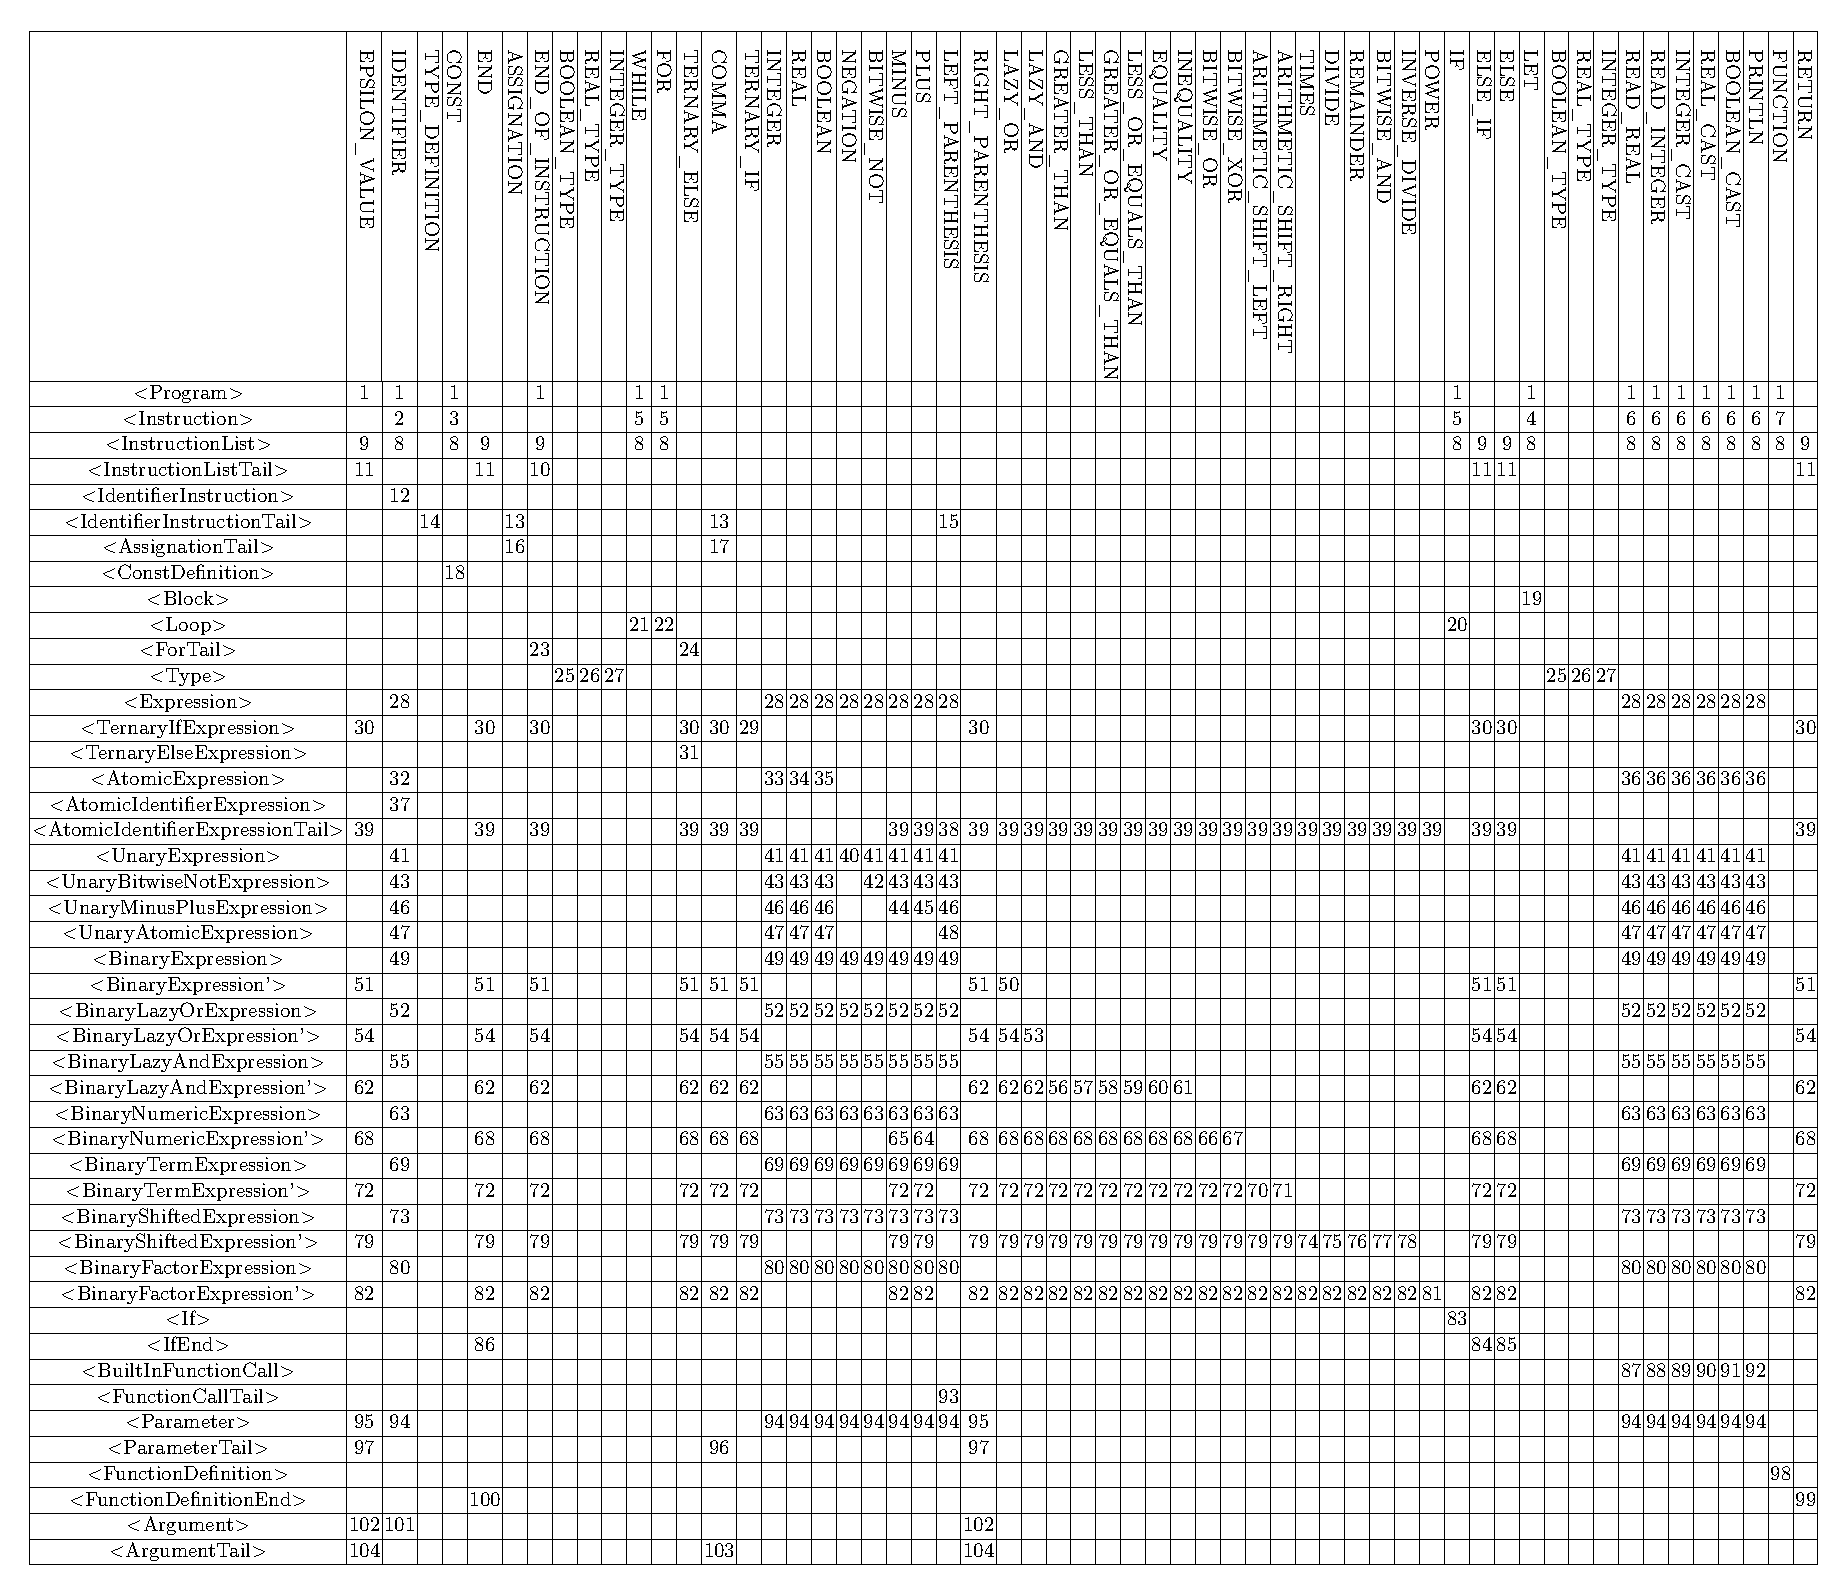
\includepdf[pages=1, angle=90]{action-table.pdf}
\end{figure}
\clearpage

\section{Génération de code}
\subsection{Introduction}
Dans la génération code, la prise en charge du type réel et de la création de fonction n'a pas été faite car non requise.\\
 \\
Pour la génération de code nous somme passé par un parser reccursif ordinaire, ce dernier appel des méthode de la classe $LlvmCodeGenerate$ qui générent le code correspodant.\\
$LlvmCodeGenerate$ possède un stack global qui permet d'y stocker des expressions, donc des variables, des valeurs entières ou booléennes.\\
Ce stack est indispenssable car toute instruction combinée doit être divisée en une série d'actions binaires, par exemple :\\
$a = 1 + 1$\\
Il faut commencer par evaluer $1 + 1$, sotcker le résultat dans une variable temporaire et puis assigner cette variable temporaire à $a$.\\
Le stack permet ici de transférer la variable temporaire.
\subsection{Structures conditionnelles}
Le $if\ else$ est déjà implémenté dans LLVM grâce une fonction qui permet de jumper à une ancre ou une autre en fonction de la valeur d'une expression booléenne.\\
Exemple:
\begin{verbatim}
def i32 compareTo ( i32 %a, i32 %b){
    entry :
        % cond = icmp slt i32 %a ,%b
        br i1 %cond , label %lower , label % greaterORequals
    lower :
        ret i32 -1
    greaterORequals :
        %1 = sub i32 %a ,%b
        ret i32 %1
\end{verbatim}
Le $else\ if$ est une cascade de $if\ else$ ou le $else$ est une ancre vers le prochaine $if$.\\\\
Le if ternaire n'est qu'une autre façons d'écrire un if.
\subsection{Boucles}
La boucle $while$ fonctionne en utilisant trois ancres, une pour le test de la condition, une pour le coeur de la boucle et une pour sortir de la boucle.\\
On commence par tester la condition, si elle est fause on saute à la fin de la boucle, si elle est vraie on saute au coeur de la boucle, une fois celle ci terminée, on saute au test de la condition.\\\\
La boucle $for$ est une autre façons d'écrire une boucle $while$ en définnisant une variable avec une valeur de base qui permettra de définir la condition de la boucle, celle ci est que cette valeur de base doit être inférieure à un maximum défini par l'utilisateur.\\
Enfin, après avoir éxecuter le coeur de la boucle il faut incrémenter la valeur de base par un nombre défini lui aussi par l'utilisateur et puis sauter au test de la condition de la boucle.

\end{document}
